\begin{appendices}
%\section*{Bijlage A}
%\addcontentsline{toc}{section}{Bijlage A}  

\newpage

\begin{landscape}
\section{OSLO ontology}
    \begin{figure}[H]
    \centering
    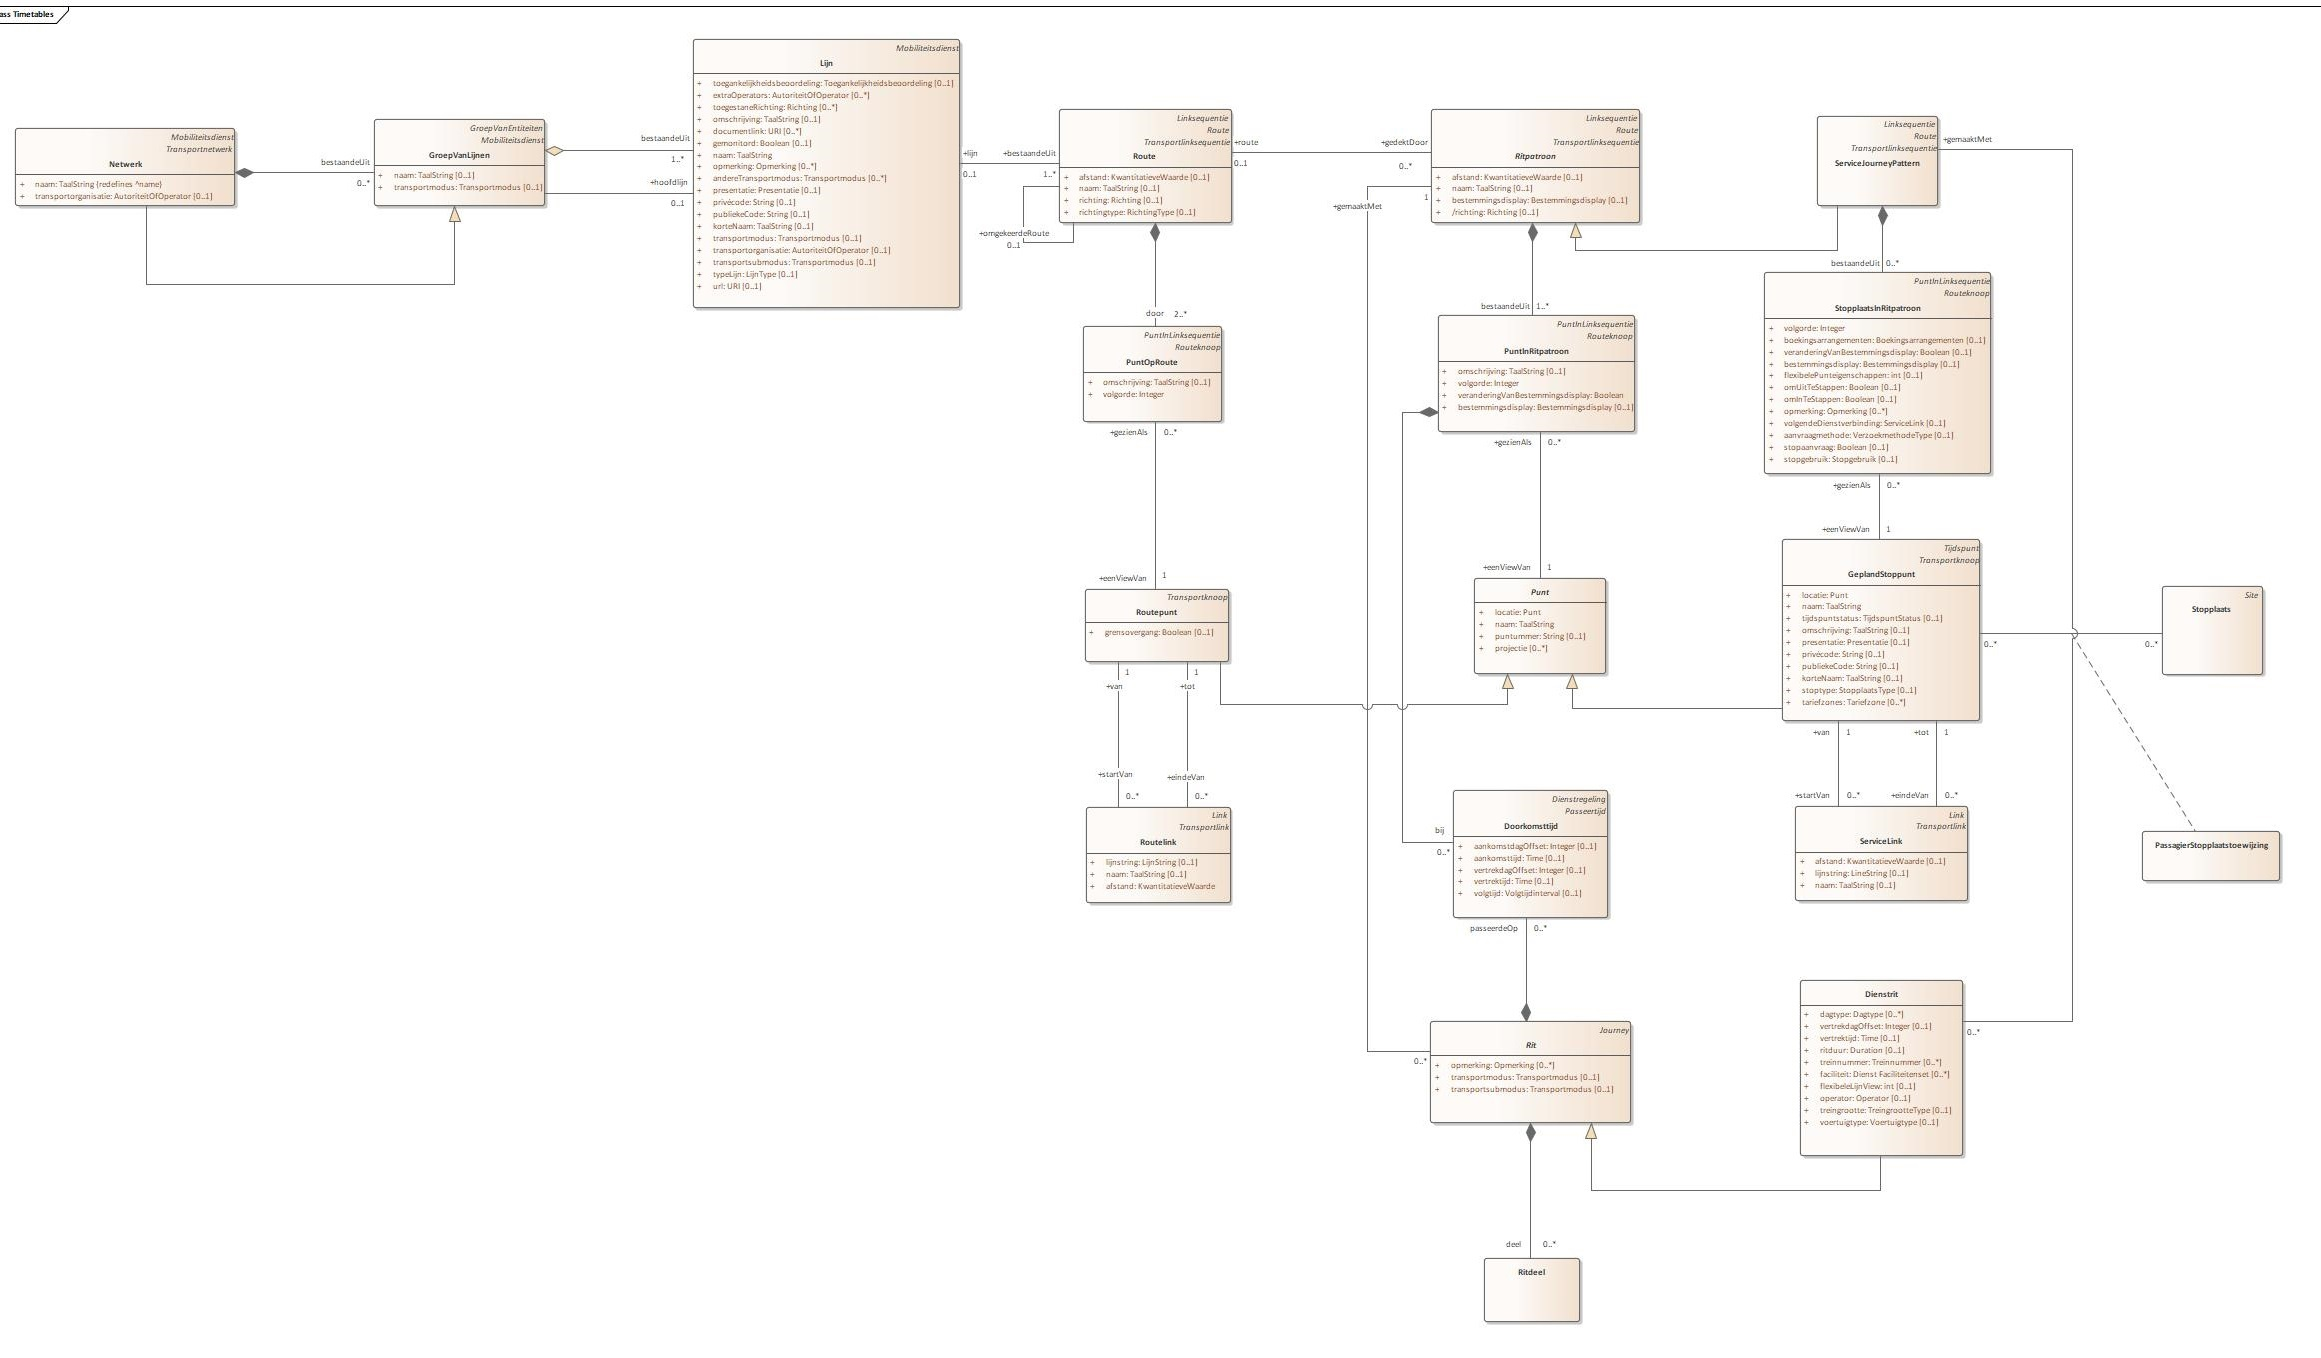
\includegraphics[width=1.4\textwidth]{images/overview.jpg}
    \caption{An small overview of the most important classes in the OSLO Mobility: timetable and route planning algorithm. }
    \tiny For a more complete overview go to \url{https://data.vlaanderen.be/doc/applicatieprofiel/mobiliteit/dienstregeling-en-planning/tijdstabellen/#introduction}
    \label{fig:appendix:Ontology:oslo:overview}
\end{figure}
\end{landscape}

\section{out of scope}
\addcontentsline{toc}{section}{Bijlage A: out of scope} 
\subsection*{SIRI}
SIRI provides an abstract model of common public transport concepts and data structures that enables the exchange of information on transport operations between different computer systems. SIRI was established as a European standard in October 2006. It is a CEN (European Committee for Standardisation) Technical Standard.

 Identification of Fixed Objects in Public Transport (incorporated into transmodel v6)
The project developed a logical data model for the fixed objects relevant for public transport, particularly for stops and points of interest. Transmodel v5.1 has been a fundamental input. IFOPT has been revised and incorporated into Transmodel v6 – Part 2.

\end{appendices}